\documentclass[11pt, a4paper]{COMP3711}
\usepackage{verbatim}
\usepackage{fancyhdr}
\usepackage{booktabs}
\usepackage{setspace}
\usepackage{amsmath,mathrsfs}
\usepackage{multicol}
\usepackage{amssymb}
\usepackage{graphicx}
\usepackage{caption}
\usepackage{subcaption}
\usepackage{array}
\usepackage{xcolor}
\usepackage{float}
\usepackage{enumitem}
\usepackage{mathcomp}
\usepackage{tabularx}
\usepackage{wasysym}
\usepackage{pbox}
\usepackage{tikz}
\usepackage{mathtools}
\usepackage{hyperref}
\hypersetup{hidelinks}
\usetikzlibrary{matrix}
\usepackage[normalem]{ulem}
\usepackage{multirow}
\usepackage[linesnumbered, ruled, boxed]{algorithm2e}
\SetKwRepeat{Do}{do}{while}

\title{Topic 2}
\subtitle{Divide \& Conquer}

\begin{document}
\begin{spacing}{1.5}
    
    \section{Intro: Binary Search}

    The main idea of {\rm Divide \& Conquer} is to solve a problem(such as of 
    size $n$) by breaking it into one or more smaller(size less than $n$) problems.
    We use binary search example to illustrate that.

    {\bf Problem:} given an {\bf sorted} array of length $n$, how to find 
    the position of element $x$; if $x$ does not exist
    in the array, output nil.

    Since the array is already sorted, it has a good property that:
    {\bf for each item $a_i$, those who are larger than $a_i$ must be 
    on its right side, while smaller than $a_i$ must be on its left side.}
    Hence we come up with an idea that we check the middle item $mid$ first,
    then we will be able to know which direction to go: left or right,
    depending on the comparison of $mid$ and $x$(the item we're looking for).
    If we go left, then the right half will be directly abandoned.
    Then we continue this process, check middle item each time, and 
    abandon half items each time.

    \begin{algorithm*}
        \caption{BinarySearch($a[]$, $left$, $right$, $x$)}
        \KwData{$a[]$: the array given, $x$: the item to find}
        \eIf{$left=right$}{
            \eIf{$a[left]=x$}{
                return $left$
            }{
                return {\bf nil}
            }
        }{
            $mid=\lfloor (left + right) / 2\rfloor$

            \eIf{$x\le a[mid]$} {
                BinarySearch($a[]$, $left$, $mid$, $x$)
            }{
                BinarySearch($a[]$, $mid+1$, $right$, $x$)
            }
        }
    \end{algorithm*}

    {\bf First call:} BinarySearch($a[]$, 1, $n$, $x$).

    This algorithm is quite efficient, since each time 
    we eliminate half of the array, with one additional 
    comparison, until there is only one item left,
    when we will end the process.

    Then let's analyse its time complexity. Let $T(n)$ be the number of 
    comparisons needed for $n$ elements, then we will have
    $$T(n)=T(n/2)+1,\ T(1)=1$$.

    Solve this {\bf recurrence}:
    \begin{align*}
        T(n) &= T(n/2) + 1\\
            &= [T(n/4) + 1] + 1\\
            &= T(n/4) + 2\\
            &=\cdots\\
            &=T(n/2^{i}) + i
    \end{align*}

    This process ends when reaching $T(1)$, i.e., 
    $i=\log_2 n$, thus, $T(n)=T(1)+\log_2 n=\log_2 n + 1$.

    We can also visualize this recurrence with recursion tree:
    (image from \url{https://cs61bl.org/su21/labs/lab10/})
    \begin{center}
        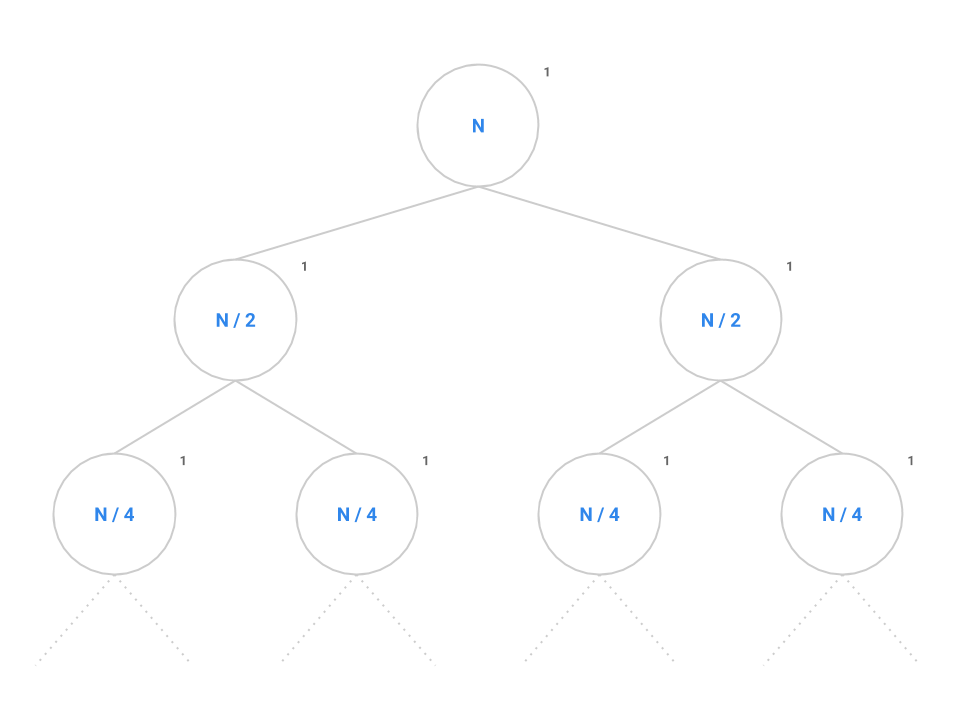
\includegraphics[scale=0.3]{images/02-bs-tree.png}
    \end{center}
    


\end{spacing}
\end{document}
